\chapter{Background}
\label{chapter: Background}

In this chapter, we introduce the fundamental concepts of mathematical programming as well as simplified forms of the models on which our modelling efforts will be built upon throughout this dissertation. This material is organised in a way that hopefully can provide the reader with a high-level understanding of the necessary mathematical concepts that will be utilised throughout this dissertation. A literature review for each topic covered has been incorporated accordingly to each section of the chapter. To gain a deeper understanding of those principles, and a more accurate grasp of the state of the art our reader is advised to thoroughly consult the literature sources referenced throughout this report.

\vspace{\baselineskip}
\noindent
Sections \ref{section: 2.1}-\ref{section: Duality} give a generic definition of Mathematical Programming, and its branches. They also mention the principal algorithms that are going to be utilised for the solution of the mathematical problems dealt with in this dissertation. Section \ref{section: vrp} studies the class of problems most relevant to the context of our problem. Sections \ref{section: Pareto}-\ref{section: Lexicographic} describe the theoretical concepts used in the latter stages of the dissertation for the experiments with the higher degree of difficulty but also the most value-added, with respect to new insights gained.

%%%%%%%%%%%%%%%%%%%%%%%%%%%%%%%%%%%%%%%%%%%%%%%%%%%%%%%%%%%%%%%%%%%%%%%%%%%%%%%%%%%    SECTION  %%%%%%%%%%%%%%%%%%%%%%%%%%%%%%%%%%%%%%%%%%%%%%%%%%%%%%%%%%%%%%%%%%%%%%

\section{Mathematical Programming}
\label{section: 2.1}
A mathematical program involves the maximizing or minimizing of an objective function by providing input values from within a defined domain, computing the value of the function that dictates the quality of each solution and subsequently choosing the best available outputs.\par
\vspace{\baselineskip}
\noindent
General mathematical programming models can be stated as \cite{DUMMY:1}:



\begin{equation}
\begin{aligned}
& \underset{x}{\text{minimise}}
& & f(x) \\
& \text{subject to}
& & g_i(x) = 0 \;\;\; i = 1,2, \ldots, m\\
& & & h_j(x) \leq 0 \;\;\; j = 1,2, \ldots, r\\
\end{aligned}
\end{equation}
\[\text{where} \; x \in S \subset \mathbb{R}^{n} \; , \; f:\mathbb{R}^{n}\rightarrow \mathbb{R} \; , \; g:\mathbb{R}^{n}\rightarrow \mathbb{R}^{m} \; \text{and} \; h:\mathbb{R}^{n}\rightarrow \mathbb{R}^{r} \]

\vspace{\baselineskip}
\noindent
The \textit{decision variables} are represented by an \textit{n}-dimensional vector  \( \pmb{x}=x_{1},x_{2}, \ldots ,x_{n} \) and the \textit{objective function f} is a function of the decision variables that we want to minimise. The \textit{feasible set}  \( S\) determined by the equations \textit{g(x)}, inequalities \textit{$h(x)$}, and set restrictions and it is a subset of the \textit{n}-dimensional space containing all the admissible decisions. All the points $x \in S$ are feasible solutions, but sought after is an optimal solution, a vector $\pmb{x^\ast}$ that satisfies the constraints of the feasible set, and achieves the best possible outcome i.e.: \par

\begin{equation*}
\begin{aligned}
f(x)\geq f(x^\ast) > -\infty \;\; \forall \; x\in S
\end{aligned}
\end{equation*}

\vspace{\baselineskip}
\noindent
The objective of mathematical programming is to utilise optimisation theory, and algorithms to obtain those optimal solution(s).


%%%%%%%%%%%%%%%%%%%%%%%%%%%%%%%%%%%%%%%%%%%%%%%%%%%%%%%%%%%%%%%%%%%%%%%%%%%%%%%%%%%    SECTION  %%%%%%%%%%%%%%%%%%%%%%%%%%%%%%%%%%%%%%%%%%%%%%%%%%%%%%%%%%%%%%%%%%%%%%

\subsection{Linear Programming}
\label{section: LP}
A\textit{ Linear Program (LP) }is a type of mathematical program where the\textbf{ }objective function and the constraints are \textbf{linear} over the feasible set of decision variables. The conventional form for representing LPs is the \textit{standard form} below \cite{DUMMY:1}:\par

\vspace{\baselineskip}

\begin{equation}
\begin{aligned}
\label{equation: LP}
& \underset{x}{\text{minimise}}
& & c_{1}x_{1}+ c_{2}x_{2}+ \ldots + c_{n}x_{n} \\
& \text{subject to}
& & a_{11}x_{1}+ a_{12}x_{2}+ \ldots + a_{1n}x_{n}=~ b_{1}\\
& & & a_{21}x_{1}+ a_{22}x_{2}+ \ldots + a_{2n}x_{n}=~ b_{2}\\
& & & \vdots\\
& & & a_{m1}x_{1}+ a_{m2}x_{2}+ \ldots + a_{mn}x_{n}=~ b_{m}\\
& \text{and}
& & x_{1},x_{2}, \ldots ,x_{n} \geq 0\\
\end{aligned}
\end{equation}
\[\text{where}~b_{i},c_{i}~\text{and}~a_{ij}~  \text{are fixed real constants and we require that} \; b_{i} \geq 0\]

\vspace{\baselineskip}
\noindent
In principle, formulating the program as a maximisation problem is equivalent to equation (\ref{equation: LP}) since through the simple transformation of the objective $maxf(x)=-min(-f(x))$ we can convert our problem. However, by convention the minimisation formulation in (\ref{equation: LP}) has prevailed, and one can transform any maximisation problem into a minimisation one without any loss of generality. The purpose of establishing a \textit{standard form} for all LPs is to create a default version that represents the standard for all LP formulations for which we can develop efficient solution algorithms. All differently formulated LPs can then be transformed to this \textit{standard form} through a series of simple operations such as the addition of slack, surplus variables so that we can utilise the effectiveness of the \textit{standard form's} universal algorithms. The formulation (\ref{equation: LP}) above can also be reduced in vector notation to this compact version:

\vspace{\baselineskip}
\begin{equation}
\label{equation: LP compact form}
\begin{aligned}
& \underset{x}{\text{minimise}}
& & c^{T}x \\
& \text{subject to}
& & Ax=b\\
& & & x \geq 0 \\
\end{aligned}
\end{equation}
\[\text{where} \; b \geq 0 \; \text{and} \; A \in \mathbb{R}^{m \times n}, \; b \in \mathbb{R}^{m \times 1}, \; c \in \mathbb{R}^{1 \times n}\]

\vspace{\baselineskip}
\noindent
A program of any scientific interest is \textit{well-defined,} and its feasible set is concretely \textbf{bounded} and \textbf{non-empty}. For LPs the feasible set circumscribed by the set of linear constraints, translates to a \textbf{convex polyhedron} containing an infinite number of solutions. According to the \textit{Fundamental Theorem of LP}, at least one of the vertices of the polyhedron feasible set, contains the optimum solution to the LP\textbf{.}\par
\vspace{\baselineskip}
\noindent
Consequently, an initial idea of an algorithm that obtains the optimal solution from inside the feasible set is the procedure of examining which of the finite number of vertices of the polyhedron \textit{S} produces the best objective value. However, computing the optimum through a \textit{finite search} over all the vertices is usually computationally prohibitive especially since the number of vertices increases exponentially [notesref] with the number of constrains and variables.\par

\todo{notesref}

%%%%%%%%%%%%%%%%%%%%%%%%%%%%%%%%%%%%%%%%%%%%%%%%%%%%%%%%%%%%%%%%%%%%%%%%%%%%%%%%%%%   SUB SECTION  %%%%%%%%%%%%%%%%%%%%%%%%%%%%%%%%%%%%%%%%%%%%%%%%%%%%%%%%%%%%%%%%%%%

\subsubsection*{Simplex Algorithm}
To combat this the \textit{Simplex Algorithm}, the most frequently used method, starts from an initial corner point and then inspects a fraction of all possible vertices \textit{pivoting} from the initial vertex to vertices with a guaranteed ever-improving objective value, until the optimum is found \cite{DUMMY:3}. Despite its effectiveness in obtaining a solution the simplex is not guaranteed to solve an LP in \textit{polynomial} time, especially considering that in some cases it is equally as hard to find an initial corner point as it is to find the optimum solution \cite{DUMMY:2}. \par

%%%%%%%%%%%%%%%%%%%%%%%%%%%%%%%%%%%%%%%%%%%%%%%%%%%%%%%%%%%%%%%%%%%%%%%%%%%%%%%%%%%   SUB SECTION  %%%%%%%%%%%%%%%%%%%%%%%%%%%%%%%%%%%%%%%%%%%%%%%%%%%%%%%%%%%%%%%%%%%

\subsubsection*{Interior point methods}

Another class of algorithms used to deal with LPs is that of \textit{interior point methods} such as \textit{Karmarkar’s Algorithm.} In contrast to the simplex, it explores the interior of the feasible space rather focusing on its corner points and identifies an optimum solution in \textit{polynomial }time \cite{DUMMY:4}.\par

%%%%%%%%%%%%%%%%%%%%%%%%%%%%%%%%%%%%%%%%%%%%%%%%%%%%%%%%%%%%%%%%%%%%%%%%%%%%%%%%%%%    SECTION  %%%%%%%%%%%%%%%%%%%%%%%%%%%%%%%%%%%%%%%%%%%%%%%%%%%%%%%%%%%%%%%%%%%%%%

\subsection{Integer Linear Programming}

A \textit{Pure-Integer Linear Program (PILP)} is a branch of linear mathematical programming in which decision variables are required to be non-negative integers.

\vspace{\baselineskip}
\begin{equation}
\begin{aligned}
& \underset{x}{\text{minimise}}
& & c^{T}x \\
& \text{subject to}
& & Ax=b\\
& & & x \geq 0, \;\;\; &x \in S \subset \mathbb{Z}^{n} \subset \mathbb{R}^{n}
\end{aligned}
\end{equation}
\[\text{where} \; b \geq 0 \; \text{and} \; A \in \mathbb{R}^{m \times n}, \; b \in \mathbb{R}^{m \times 1}, \; c \in \mathbb{R}^{1 \times n}\]

\vspace{\baselineskip}
\noindent
A visualisation of the feasible set of a program that includes the integrality constraint can be seen in Figure \ref{fig:Integer Programming figure}. Assuming, that we consider an integer problem for which  $\pmb{x} \in \mathbb{Z}^{2}$, Figure \ref{fig:Integer Programming figure}(a) illustrates the spectrum of possible decisions that we can make for this problem. Those decision are the subset of integer pairs that belong in $S$.

\vspace{\baselineskip}
\noindent
In a \textit{Mixed Integer Linear Program (MILP)} only a subset of the decision variables have an integrality constraint. Taking as an example the two-dimensional MILP of Figure \ref{fig:Integer Programming figure}(b) in which one decision variable is continuous ($x_1 \in \mathbb{R}$) whereas the other can only take discrete values ($x_2 \in \mathbb{Z}$).\par

\vspace{\baselineskip}
\noindent
Many real-life problems can be formulated as integer linear programs. The study of this class of programs and its algorithms is particularly important for the purposes of this dissertation since we will be formulating our problem as a MILP. In particular, the problem that we will be studying from Chapter \ref{chapter: Problem Definition} onward, is a Binary Mixed-Integer Program where binary discrete variables are used to model whether or not some event takes place.\par

 \vspace{\baselineskip}
\noindent
In reality, even though it seems slightly counter-intuitive at first, integer programs are considerably harder to solve. A naive assumption would be to claim that in an ILP, one only has a finite number of possible decisions (as seen in Figure \ref{fig:Integer Programming figure}(a)) so in principle one could essentially try them all. However, if the problem's scale is increased we will transition to a combinatorial problem where the number of solutions that one has to search over with this brute force approach becomes very large very quickly. We mentioned before that in the environment of LPs when we add new constraints the number of solutions increases exponentially. In an ILP specifically, the addition of \textit{n} binary variables increases the solution space by 2\textsuperscript{n}. As a consequence, a \textit{polynomial }time algorithm for ILPs has not yet been proven to exist \cite{DUMMY:2}, and such MILPs are considered \textit{NP-hard} \cite{Wedelin1995}.

\vspace{\baselineskip}
\noindent
To solve mixed-integer linear problems, we can either reuse or extend algorithms designed for LPs or construct new ones specifically for ILP problems. The algorithms studied below are of the former category and they largely exploit the efficiency of the simplex algorithm\footnote{Designed for standard form LPs as was previously seen in Section \ref{section: LP}.} by disentangling an integer LP into a corresponding linear program through relaxing\footnote{The concept of obtaining the relaxation of a program is further explained in Appendix \ref{section: Appednix Relaxation} for interested readers.} the integrality constraints. 

\vspace{\baselineskip}
\noindent
This approach is based on the idea that the ILP’s feasible set is a subset of the relaxed LP’s domain\footnote{$S_{ILP}$ $\subseteq$ $S_{R}$, where $S_{R}$ is the relaxed LP's feasible set.}, hence the integer optimum solution is guaranteed to be contained within the linear spectrum of solutions. Subsequently, through solving numerous iterations of the \textit{standard form} LPs, utilising simplex, their feasible sets are gradually modified to converge towards an optimum solution that is also integer hence, obtaining a solution that is also the optimal for the original ILP. The reason for multiple such algorithms to exist is revolved around the way they modify the relaxed LPs feasible set to converge towards the integer solution. \par

%%%%%%%%%%%%%%%%%%%%%%%%%%%%%%%%%%%%%%%%%%%%%%%%%%%%%%%%%%%%%%%%%%%%%% DOUBLE Figure %%%%%%%%%%%%%%%%%%%%%%%%%%%%%%%%%%%%%%%%%%%%%%%

%Two images in one, illustrating atomic block
\begin{figure}%
    \centering
    \subfloat[Pure-Integer Linear Programming problem (PILP), where $\pmb{x} \in \mathbb{Z}^{2}$.]{
    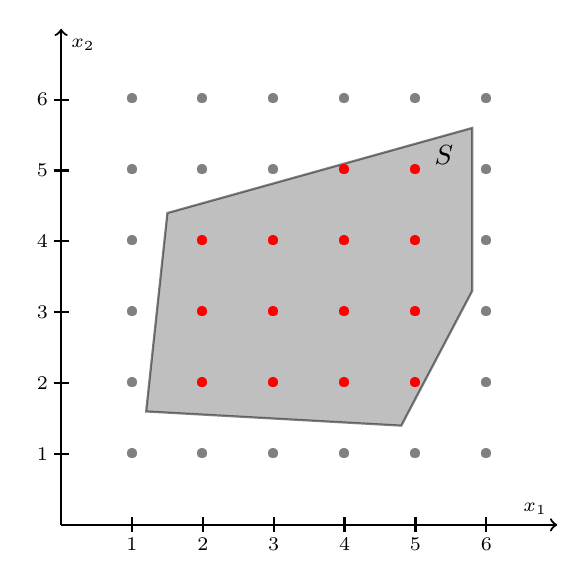
\begin{tikzpicture}[thick, scale=0.9]
    \begin{scope}[thick,font=\scriptsize]
    % Axes:
    % Are simply drawn using line with the `->` option to make them arrows:
    % The main labels of the axes can be places using `node`s:
    \draw [->] (0,0) -- (7,0) node [above left]  {$x_1$};
    \draw [->] (0,0) -- (0,7) node [below right] {$x_2$};
    
    %dotted lines
    %edge points
    %\draw [dashed] (4,0) -- (4,1);
    %\draw [dashed] (0,3) -- (2,3);
    

    % Axes labels:
    % Are drawn using small lines and labeled with `node`s. The placement can be set using options
    \iffalse% Single
    % If you only want a single label per axis side:
    \draw (1,-3pt) -- (1,3pt)   node [above] {$1$};
    \draw (-3pt,1) -- (3pt,1)   node [right] {$1$};
    
    \else% Multiple
    % If you want labels at every unit step:
    \foreach \n in {1,2,...,5,6}{%
        \draw (\n,-3pt) -- (\n,3pt)   node [label=below:$\n$] {};
        \draw (-3pt,\n) -- (3pt,\n)   node [label=left:$\n$] {};
    }
    \fi
    \end{scope}
    % The circle is drawn with `(x,y) circle (radius)`
    % You can draw the outer border and fill the inner area differently.
    % Here I use gray, semitransparent filling to not cover the axes below the circle
   % \path [draw=skiastro,fill=skiastro,semitransparent] (+3,+3) circle (2);1
    
     \node[label=right:] (F) at (4.8,1.4){};
     \node[label=below:] (A) at (1.2,1.6){};
     \node[label=right:] (X) at (5.8,5.6){};
     \node[label=right:] (C) at (5.8,3.3){};
     \draw[thick,fill=gray,semitransparent] (1.5,4.4)  %fills up the figure
     to[bend right=0] (X.center) 
     to[bend left=0] (C.center)
     to[bend left=0] (F.center) 
     to[bend left=0] (A.center) to[bend left=0]  cycle;
    
    % Place the labels of the circle:
    % edge points
 %   \node [below right,darkgray] at (+4,1) {$\pmb{minf_1}$};
%    \node [above left,darkgray] at (2,3) {$\pmb{minf_2}$};
    

    
    %Red points
    %draw edge points
%     \node at (2,3) {\textcolor{red}{\textbullet}};
 %    \node at (4,1) {\textcolor{red}{\textbullet}};    
    
    \node [below,black] at (+5.4,5.5) {$S$};
    
    \node at (1,1) {\textcolor{gray}{\textbullet}};
    \node at (1,2) {\textcolor{gray}{\textbullet}};
    \node at (1,3) {\textcolor{gray}{\textbullet}};
    \node at (1,4) {\textcolor{gray}{\textbullet}};
    \node at (1,5) {\textcolor{gray}{\textbullet}};
    \node at (1,6) {\textcolor{gray}{\textbullet}};
    \node at (2,1) {\textcolor{gray}{\textbullet}};
    \node at (2,2) {\textcolor{red}{\textbullet}};
    \node at (2,3) {\textcolor{red}{\textbullet}};
    \node at (2,4) {\textcolor{red}{\textbullet}};
    \node at (2,5) {\textcolor{gray}{\textbullet}};
    \node at (2,6) {\textcolor{gray}{\textbullet}};
    \node at (3,1) {\textcolor{gray}{\textbullet}};
    \node at (3,2) {\textcolor{red}{\textbullet}};
    \node at (3,3) {\textcolor{red}{\textbullet}};
    \node at (3,4) {\textcolor{red}{\textbullet}};
    \node at (3,5) {\textcolor{gray}{\textbullet}};
    \node at (3,6) {\textcolor{gray}{\textbullet}};
    \node at (4,1) {\textcolor{gray}{\textbullet}};
    \node at (4,2) {\textcolor{red}{\textbullet}};
    \node at (4,3) {\textcolor{red}{\textbullet}};
    \node at (4,4) {\textcolor{red}{\textbullet}};
    \node at (4,5) {\textcolor{red}{\textbullet}};
    \node at (4,6) {\textcolor{gray}{\textbullet}};
    \node at (5,1) {\textcolor{gray}{\textbullet}};
    \node at (5,2) {\textcolor{red}{\textbullet}};
    \node at (5,3) {\textcolor{red}{\textbullet}};
    \node at (5,4) {\textcolor{red}{\textbullet}};
    \node at (5,5) {\textcolor{red}{\textbullet}};
    \node at (5,6) {\textcolor{gray}{\textbullet}};
    \node at (6,1) {\textcolor{gray}{\textbullet}};
    \node at (6,2) {\textcolor{gray}{\textbullet}};
    \node at (6,3) {\textcolor{gray}{\textbullet}};
    \node at (6,4) {\textcolor{gray}{\textbullet}};
    \node at (6,5) {\textcolor{gray}{\textbullet}};
    \node at (6,6) {\textcolor{gray}{\textbullet}};

    \end{tikzpicture}}%picture #1
    \qquad
    %picture #2
    \subfloat[Mixed-Integer Linear Programming problem (MILP), where $x_1 \in \mathbb{R}$ and $x_2 \in \mathbb{Z}$.]{
            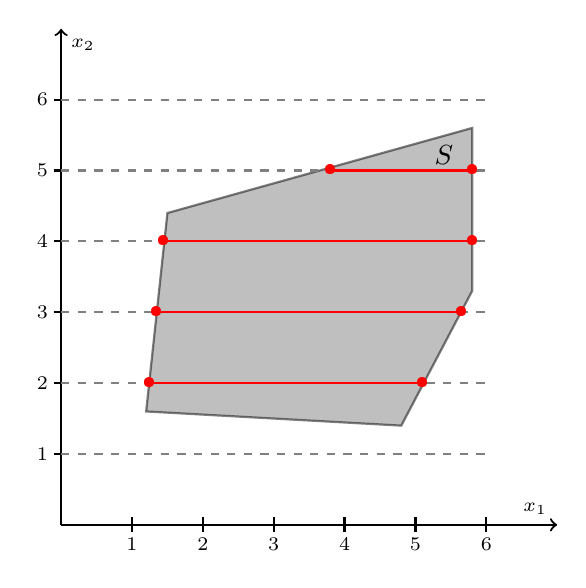
\begin{tikzpicture}[thick, scale=0.9]
    \begin{scope}[thick,font=\scriptsize]
    % Axes:
    % Are simply drawn using line with the `->` option to make them arrows:
    % The main labels of the axes can be places using `node`s:
    \draw [->] (0,0) -- (7,0) node [above left]  {$x_1$};
    \draw [->] (0,0) -- (0,7) node [below right] {$x_2$};
    
    %dotted lines
    %edge points
    %\draw [dashed] (4,0) -- (4,1);
    %\draw [dashed] (0,3) -- (2,3);
    

    % Axes labels:
    % Are drawn using small lines and labeled with `node`s. The placement can be set using options
    \iffalse% Single
    % If you only want a single label per axis side:
    \draw (1,-3pt) -- (1,3pt)   node [above] {$1$};
    \draw (-3pt,1) -- (3pt,1)   node [right] {$1$};
    
    \else% Multiple
    % If you want labels at every unit step:
    \foreach \n in {1,2,...,5,6}{%
        \draw (\n,-3pt) -- (\n,3pt)   node [label=below:$\n$] {};
        \draw (-3pt,\n) -- (3pt,\n)   node [label=left:$\n$] {};
    }
    \fi
    \end{scope}
    % The circle is drawn with `(x,y) circle (radius)`
    % You can draw the outer border and fill the inner area differently.
    % Here I use gray, semitransparent filling to not cover the axes below the circle
   % \path [draw=skiastro,fill=skiastro,semitransparent] (+3,+3) circle (2);1
    
     \node[label=right:] (F) at (4.8,1.4){};
     \node[label=below:] (A) at (1.2,1.6){};
     \node[label=right:] (X) at (5.8,5.6){};
     \node[label=right:] (C) at (5.8,3.3){};
     \draw[thick,fill=gray,semitransparent] (1.5,4.4)  %fills up the figure
     to[bend right=0] (X.center) 
     to[bend left=0] (C.center)
     to[bend left=0] (F.center) 
     to[bend left=0] (A.center) to[bend left=0]  cycle;
    
    % Place the labels of the circle:
    % edge points
 %   \node [below right,darkgray] at (+4,1) {$\pmb{minf_1}$};
%    \node [above left,darkgray] at (2,3) {$\pmb{minf_2}$};
    

    
    %Red points
    %draw edge points
%     \node at (2,3) {\textcolor{red}{\textbullet}};
 %    \node at (4,1) {\textcolor{red}{\textbullet}};    
    
    \node [below,black] at (+5.4,5.5) {$S$};
    
    \draw [gray, dashed] (0,1) -- (6,1);
    \draw [gray, dashed] (0,2) -- (6,2);
    \draw [red, thick] (1.25,2) -- (5.1,2);
    \node at (1.25,2) {\textcolor{red}{\textbullet}};
    \node at (5.1,2) {\textcolor{red}{\textbullet}};
    \draw [gray, dashed] (0,3) -- (6,3);
    \draw [red, thick] (1.4,3) -- (5.6,3);
    \node at (1.35,3) {\textcolor{red}{\textbullet}};
    \node at (5.65,3) {\textcolor{red}{\textbullet}};
    \draw [gray, dashed] (0,4) -- (6,4);
    \draw [red, thick] (1.45,4) -- (5.8,4);
    \node at (1.45,4) {\textcolor{red}{\textbullet}};
    \node at (5.8,4) {\textcolor{red}{\textbullet}};
    \draw [gray, dashed] (0,5) -- (6,5);
    \draw [red, thick] (3.8,5) -- (5.8,5);
    \node at (3.8,5) {\textcolor{red}{\textbullet}};
    \node at (5.8,5) {\textcolor{red}{\textbullet}};
    \draw [gray, dashed] (0,6) -- (6,6);

    \end{tikzpicture}}
    %end of picture #2
    \caption{Illustrations of the Feasible Sets ($S$) of an ILP and a MILP respectively.}%
    \label{fig:Integer Programming figure}%
\end{figure}

%%%%%%%%%%%%%%%%%%%%%%%%%%%%%%%%%%%%%%%%%%%%%%%%%%%%%%%%%%%%%%%%%%%%%%%%%%%%%%%%%%%   SUB SECTION  %%%%%%%%%%%%%%%%%%%%%%%%%%%%%%%%%%%%%%%%%%%%%%%%%%%%%%%%%%%%%%%%%%%

\subsubsection*{Branch and Bound}
The \textit{Branch and Bound (BB)} follows this philosophy of modifying the feasible set until an integer solution is obtained. It begins by obtaining the optimum solution of the relaxed LP. In the case that this initial solution happens to be integer it will immediately terminate since that will mean that the optimum for the original ILP has also been found. If it is not however, the algorithm modifies the LP’s feasible set until its solution satisfies the integrality constraints. \par

\vspace{\baselineskip}
\noindent
Those modifications take place at every iteration, and for the purposes of the BB we refer to them as \textit{branching}. To carry out branching the algorithm divides the solution space into two LP subproblems, by eliminating a part of the LP relaxation’s feasible set that did not contain any feasible integer solutions. For the ILP there is no loss of generality since the union of the subproblems’ feasible sets contains the exact same feasible integer solutions. The two emergent subproblems are then solved separately as regular LPs. Due to the absence of any loss of generality the optimum ILP solution is guaranteed to be in just one of the two new emergent solution spaces of the subproblems. If the solution to either of the two subproblems is worse than any previously known solution, then the corresponding subproblem and its feasible space are disregarded as non-promising. This is known as the \textit{fathoming} step. In essence through such iterations of the algorithm a lower possible bound for the objective value is eventually obtained. \par

\vspace{\baselineskip}
\noindent
By enforcing these two steps iteratively, a binary tree is constructed. Nodes with a non-integer solution have two branching subproblems et cetera. The algorithm is terminated when all nodes will either have an integer solution or a non-integer solution that is worse than the best integer solution of some other node. The node with the most optimum integer solution is the solution to the original ILP \cite{DUMMY:2}.   \par

%%%%%%%%%%%%%%%%%%%%%%%%%%%%%%%%%%%%%%%%%%%%%%%%%%%%%%%%%%%%%%%%%%%%%%%%%%%%%%%%%%%   SUB SECTION  %%%%%%%%%%%%%%%%%%%%%%%%%%%%%%%%%%%%%%%%%%%%%%%%%%%%%%%%%%%%%%%%%%%

\subsubsection*{Cutting Plane}
The \textit{Cutting Plane (CP)} method is also concerned with the transformation of an ILP into a LP that has naturally an integer solution. The process behind this is to gradually cut out part of the relaxed LP's admissible set while leaving the feasible region of the ILP completely unchanged. Hence, eventually upon the implementation of a sufficient number of such \textit{cuts} we will obtain an LP with an integer solution. However, the process of generating the cuts is not a trivial task, and that is the heart of the algorithm. 

\vspace{\baselineskip}
\noindent
The algorithm starts by relaxing the integrality constraints to obtain the LP relaxation of the original ILP. Starting from the optimum solution of the LP relaxation, if it is integer, then the \textit{cutting-plane} algorithm terminates, and this optimum solution is also optimum for the ILP. If it is not, we \textit{tighten} the feasible set of the LP and repeat this process. \par
\vspace{\baselineskip}
\noindent
The \textit{tightening }is done by generating a \textit{cut,} that is a new constraint that restricts unwanted non-integer solutions. This new linear constraint is added to the relaxed LP’s solution space hence modifying $S_{R}$ into a new set $S_{CH}$. This process of modifying $S_{R}$ is repeated until the set converges to one of the ILP’s solution space vertices, at which point the optimum integer solution will have been obtained. Through iteratively performing these steps we create the \textit{convex hull} $S_{CH}$ of the ILP's feasible set $S$.\par

\vspace{\baselineskip}
\noindent
Consequently, starting from the ILP below:

\begin{equation*}
\begin{aligned}
& \underset{x}{\text{minimise}}
& & c^{T}x, \;\;\;\; x \in S \\
\end{aligned}
\end{equation*}

\vspace{\baselineskip}
\noindent
Through generating multiple cuts at each iteration we can instead solve:

\begin{equation*}
\begin{aligned}
& \underset{x}{\text{minimise}}
& & c^{T}x, \;\;\;\; x \in S_{CH} \\
\end{aligned}
\end{equation*}
\[\text{since} \; S \subseteq S_{CH} \subseteq S_{R} \]


\vspace{\baselineskip}
\noindent
The ideal operating scenario for this method would be to generate a relatively small account of highly effective cuts. However, the effectiveness of a cut is a topic with a hard to obtain answer. A universally good cut, would be a cut where the vertex of $S_{CH}$ on which the cut is performed is the furthest from the perimeter of $S_{R}$ since that would automatically mean that the largest possible amount of unwanted feasible space has been cut off. In order generate such good cuts, the simplex algorithm can be utilised. Namely, at each iteration after locating a vertex, we can use the simplex algorithm at that point to determine the best point to pivot to in order to perform the following cut \cite{ieeeeee}.

\vspace{\baselineskip}
\noindent
Overall, a pure cutting plane approach is considered computationally intensive because more often than not, multiple cuts are required. As a direct consequence multiple constraints will be added to the LP relaxation rendering it less computationally tractable. Especially, if we consider that the number of cuts required is not necessarily dependent on the problem’s scale as explained in \cite{DUMMY:3}. In general, there also exist many kinds of cuts such as \textit{Mixed-Integer rounding, }or \textit{Knapsack cover }cuts derived from the logic governing the class packing problems. This adds another variable to the algorithm regarding the choice of cuts. The most prominent are \textit{Gomory mixed-integer }cuts \cite{gomory1958}. Although at the time of their development they were unable to translate their theoretical effectiveness into practice they have recently been revisited and are now considered a go-to method. That is due to the following two reasons. Firstly, due to the emergence of more powerful and robust solvers \cite{cornelio}. Secondly, they have proven to outperform other methods when utilised with a hybrid implementation of the cutting algorithm instead of the pure cutting plane approach. Namely, when utilised a method that combines the \textit{branch-and-bound} with the \textit{cutting-plane} algorithm (i.e. a \textit{branch-and-cut})\cite{BALAS19961} they manage to generate substantially better bounds leading to a decreased computation time compared to the pure versions of those two algorithms \cite{DUMMY:2}.\par

%%%%%%%%%%%%%%%%%%%%%%%%%%%%%%%%%%%%%%%%%%%%%%%%%%%%%%%%%%%%%%%%%%%%%%%%%%%%%%%%%%%    SECTION  %%%%%%%%%%%%%%%%%%%%%%%%%%%%%%%%%%%%%%%%%%%%%%%%%%%%%%%%%%%%%%%%%%%%%%

\subsection*{Duality}
\label{section: Duality}

According to the principle of \textit{duality, }in linear programming every LP can be associated with a corresponding \textit{dual} linear program. The \textit{dual} of a problem is a LP derived from combinations of the constraints of an original LP model, referred to as the \textit{primal.} The solution of the \textit{dual} signifies the best possible bound of the original problem. In matrix form, we can express the \textit{primal} problem as:\par

\vspace{\baselineskip}
\begin{equation*}
\begin{aligned}
& \underset{x}{\text{minimise}}
& & c^{T}x \\
& \text{subject to}
& & Ax \leq b\\
& & & x \geq 0 \\\
\end{aligned}
\end{equation*}

\noindent
with the corresponding \textbf{symmetric} dual problem,\par

\vspace{\baselineskip}
\begin{equation*}
\begin{aligned}
& \underset{x}{\text{minimise}}
& & b^{T}y \\
& \text{subject to}
& & A^{T}y \geq c\\
& & & x \geq 0 \\\
\end{aligned}
\end{equation*}

\noindent
The two problems are completely intertwined with each other. The objective of the primal program is transformed to its mirror-image counterpart in the dual, in a way that if the original is a minimisation problem its dual attempts to maximise the objective function and vice versa. Finding the dual of the dual problem will lead us back to the primal problem. \par
\vspace{\baselineskip}
\noindent
In Linear Programming specifically, the concept of \textit{strong duality }states that the optimum solution to the dual problem is also the optimum for the primal and vice versa. We can leverage this concept when solving LPs where the number of variables is significantly smaller than that of the constraints, since solving the dual will be considerably more computationally efficient and its solution will also be optimum for the original problem. \par

\vspace{\baselineskip}
\noindent
A practical use of the duality concept is that it drives the \textit{post-optimal analysis, }to determine the degree of sensitivity of the optimum solution to any changes in the input parameters. \par

%%%%%%%%%%%%%%%%%%%%%%%%%%%%%%%%%%%%%%%%%%%%%%%%%%%%%%%%%%%%%%%%%%%%%%%%%%%%%%%%%%%   SUB SECTION  %%%%%%%%%%%%%%%%%%%%%%%%%%%%%%%%%%%%%%%%%%%%%%%%%%%%%%%%%%%%%%%%%%%
\subsubsection*{Sensitivity Analysis}

Sensitivity Analysis leverages the relationship between primal-dual problems to calculate the changes in the optimum solution as a result of changes in the input parameters, in an efficient manner. The utility of performing a sensitivity analysis is to gain insights of the relationships between the various components of the problem. For instance, in chapter \ref{chapter: Problem Definition} we will conduct a sensitivity analysis to find out the various the trade-off between the objective function and a variable of the problem. By probing the objective function for various values of that variable we are able to determine the thresholds at which the objective value changes as well as the degree by which it changes. Finally, while performing a sensitivity analysis it is often useful to determine the degree to which a component can remain robust with respect to some changes in another component. For instance, we could establish limits within which changing a certain variable will not cause a change in the optimal solution. Consequently, having done that we will have determined the sensitivity of the optimal solution to changes with respect to that variable.\par

%%%%%%%%%%%%%%%%%%%%%%%%%%%%%%%%%%%%%%%%%%%%%%%%%%%%%%%%%%%%%%%%%%%%%%%%%%%%%%%%%%%   SUB SECTION  %%%%%%%%%%%%%%%%%%%%%%%%%%%%%%%%%%%%%%%%%%%%%%%%%%%%%%%%%%%%%%%%%%%

\subsubsection*{Lagrangian Relaxation}
\addcontentsline{toc}{paragraph}{Lagrangian Relaxation}
The \textit{Lagrangian dual} problem is a bounding technique for solving ILPs that does not disregard the integrality constraints as in previously stated techniques, but instead relaxes some of the main constraints. By forming a combination of the constraints through multiplying them with non-negative Lagrange multipliers, the dual of the original ILP is constructed. The relaxed problem is significantly more computationally tractable, and through solving the dual we can establish a best possible bound for the original ILP.\par

%%%%%%%%%%%%%%%%%%%%%%%%%%%%%%%%%%%%%%%%%%%%%%%%%%%%%%%%%%%%%%%%%%%%%%%%%%%%%%%%%%%    SECTION  %%%%%%%%%%%%%%%%%%%%%%%%%%%%%%%%%%%%%%%%%%%%%%%%%%%%%%%%%%%%%%%%%%%%%%

\section{Multi-Objective Optimisation and Pareto Optimality}
\label{section: Pareto}
Taking a brief diversion from the context of Linear Programming, we look at \textit{Multi-Objective Optimisation} problems where the objective function is comprised of a multitude of objectives. For such problems the \textit{Pareto Optimality} principle proves particularly handy when looking for a \textbf{Pareto optimal} solution. In simple terms To define a Pareto optimal solution we first need to address the concept of a \textbf{dominated solution}: 

\begin{equation}
\begin{aligned}
\label{equation: pareto}
& \underset{x}{\text{minimise}}
& & f(x) \\
& \text{subject to}
& & h_i(x) = 0 \;\;\; i = 1,2, \ldots, m\\
\end{aligned}
\end{equation}
\[where \; x \in \mathbb{Z}^{n} \;, \; f:\mathbb{Z}^{n}\rightarrow \mathbb{Z}^{c}, \; h:\mathbb{Z}^{n}\rightarrow \mathbb{Z}^{m} \]

\vspace{\baselineskip}
\noindent
Given the constrained multi-objective minimisation problem in (\ref{equation: pareto}), that has an objective function $f(x)$ which is a combination of a set of \textit{o} objective functions $f_{1}(x),f_{2}(x),\ldots,f_{o}(x)$ that require simultaneous minimisation, and a feasible space defined by a set of constraints $m$, a feasible solution $d$ is \textbf{dominated} by another feasible solution $s$ if the following two conditions stand:


\begin{equation*}
\begin{aligned}
&(1) \; & &f_{j}(s) \leq f_{j}(d) \; \forall \; j \in [1,\dots,o] \\
&(2) \; & &\exists \; k \in [1,\dots,m] \; | \; f_{k}(s) < f_{k}(d) \\ 
\end{aligned}
\end{equation*}


\vspace{\baselineskip}
\noindent
In simpler terms, these two conditions can be reduced down to: (1) solution $s$ is \textit{as good performing as} $d$ at every objective $o$, and simultaneously, (2) solution $s$ \textbf{strictly} better performing than $d$ at at least one objective \cite{DUMMY:6}. Using the definition of a \textit{dominated} solution, we then define the Pareto optimal solutions as the set of \textbf{undominated} solutions from within the feasible set.

\vspace{\baselineskip}
\noindent
In the context of a practical optimisation problem, finding a feasible point that is concurrently Pareto optimal means that it is only impossible to improve one objective at the expense of another. Hence, it captures the concept of a \textbf{trade-off} between the various objective in the objective function. The reason behind the efficacy of this concept is that more often than not, when presented with a multi-objective optimisation problem it is usually precarious to apply the philosophy of linear programming and trying to optimise multiple objectives in a brute-force way, as it is likely that the optimiser for one of the objective is not going to coincide with that of a different objective. That is because more often than not, especially in problems with numerous objective functions, some objective functions end up being in conflict with each other \cite{grinding}. Hence, we need to address a multi-objective optimisation problem with a slightly different notion of optimality. 

%%%%%%%%%%%%%%%%%%%%%%%%%%%%%%%%%%%%%%%%%%%%%%%%%%%%%%%%%%%%%%%%%%%%%%%%%%%% FIGURE %%%%%%%%%%%%%%%%%%%%%%%%%%%%%%%%%%%%%%%%%%%%%%%%%%%%%%%%%%%%%%%%%%%%%%%%%%%%%%%%

\begin{figure}
    \centering
    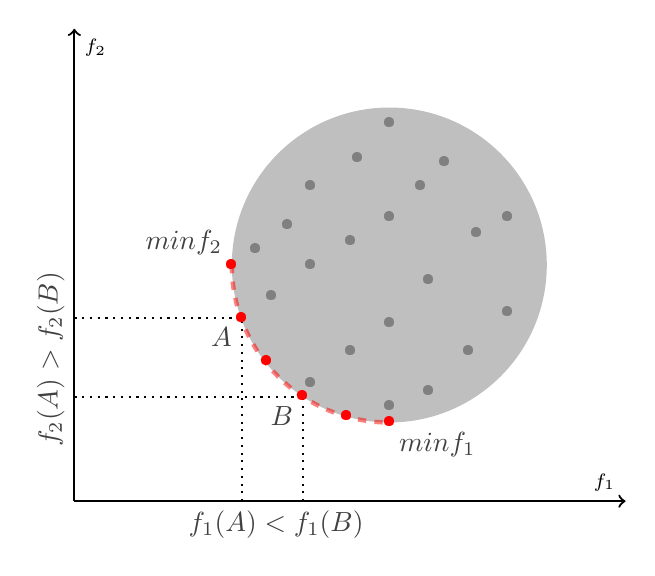
\begin{tikzpicture}
    \begin{scope}[thick,font=\scriptsize]
    % Axes:
    % Are simply drawn using line with the `->` option to make them arrows:
    % The main labels of the axes can be places using `node`s:
    \draw [->] (0,0) -- (7,0) node [above left]  {$f_1$};
    \draw [->] (0,0) -- (0,6) node [below right] {$f_2$};
    
    %dotted lines
    %edge points
    %\draw [dashed] (4,0) -- (4,1);
    %\draw [dashed] (0,3) -- (2,3);
    
    %A
    \draw [dotted] (2.125,0) -- (2.125,2.328);
    \draw [dotted] (0,2.328) -- (2.125,2.328);
    
    %B
    \draw [dotted] (2.9,0) -- (2.9,1.325);
    \draw [dotted] (0,1.325) -- (2.9,1.325);

    % Axes labels:
    % Are drawn using small lines and labeled with `node`s. The placement can be set using options
    \iffalse% Single
    % If you only want a single label per axis side:
    \draw (1,-3pt) -- (1,3pt)   node [above] {$1$};
    \draw (-3pt,1) -- (3pt,1)   node [right] {$1$};
    
    \else% Multiple
    % If you want labels at every unit step:

    \fi
    \end{scope}
    % The circle is drawn with `(x,y) circle (radius)`
    % You can draw the outer border and fill the inner area differently.
    % Here I use gray, semitransparent filling to not cover the axes below the circle
    \path [draw=none,fill=gray,semitransparent] (+4,+3) circle (2);
    \path [draw=red, ultra thick,fill=none,semitransparent, dashed] (+2,+3) arc[start angle=180, end angle=270, radius=2];
    
    % Place the labels of the circle:
    % edge points
    \node [below right,darkgray] at (+4,1) {$\pmb{minf_1}$};
    \node [above left,darkgray] at (2,3) {$\pmb{minf_2}$};
    
    %A,B
    \node [below left,darkgray] at (2.9,1.325) {$B$};
    \node [below left,darkgray] at (2.125,2.328) {$A$};
    
    \node [below,darkgray] at (2.5625,0) {$f_1(A)<f_1(B)$};
    \node [above ,darkgray,rotate=90] at (0,1.801) {$f_2(A)>f_2(B)$};
    
    %Red points
    %draw edge points
     \node at (2,3) {\textcolor{red}{\textbullet}};
     \node at (4,1) {\textcolor{red}{\textbullet}};    
     
    %draw MIDWAY points
     %\node at (2.0425,2.6) {\textcolor{red}{\textbullet}};
     \node at (2.125,2.318) {\textcolor{red}{\textbullet}}; %A
     %\node at (2.25,2.032) {\textcolor{red}{\textbullet}};
     \node at (2.435,1.777) {\textcolor{red}{\textbullet}};    
     %\node at (2.75,1.439) {\textcolor{red}{\textbullet}};    
     \node at (2.9,1.325) {\textcolor{red}{\textbullet}}; %B
     \node at (3.45,1.075) {\textcolor{red}{\textbullet}};    
     

     \node at (2.3,3.2) {\textcolor{gray}{\textbullet}};
     \node at (2.5,2.6) {\textcolor{gray}{\textbullet}};
     \node at (3,1.5) {\textcolor{gray}{\textbullet}};
     
     \node at (2.7,3.5) {\textcolor{gray}{\textbullet}};
     \node at (3,3) {\textcolor{gray}{\textbullet}};
     \node at (3.5,1.9064) {\textcolor{gray}{\textbullet}};
     \node at (4,1.2) {\textcolor{gray}{\textbullet}};

     \node at (3,4) {\textcolor{gray}{\textbullet}};
     \node at (3.5,3.3) {\textcolor{gray}{\textbullet}};
     \node at (4,2.264) {\textcolor{gray}{\textbullet}};
     \node at (4.5,1.4) {\textcolor{gray}{\textbullet}};

     \node at (3.6,4.35) {\textcolor{gray}{\textbullet}};
     \node at (4,3.6) {\textcolor{gray}{\textbullet}};
     \node at (4.5,2.8) {\textcolor{gray}{\textbullet}};
     \node at (5,1.9) {\textcolor{gray}{\textbullet}};
     
     \node at (4,4.8) {\textcolor{gray}{\textbullet}};
     \node at (4.4,4) {\textcolor{gray}{\textbullet}};
     \node at (4.7,4.3) {\textcolor{gray}{\textbullet}};
     \node at (5.1,3.4) {\textcolor{gray}{\textbullet}};
     \node at (5.5,3.6) {\textcolor{gray}{\textbullet}};
     \node at (5.5,2.4) {\textcolor{gray}{\textbullet}};

    \end{tikzpicture}
    \caption{The image of the feasible set of a Bi-Objective Optimisation problem showcasing the Pareto Front.}
    \label{fig:Pareto figure}
\end{figure}

\vspace{\baselineskip}
\noindent
Suppose, we are given a constrained multi-objective optimisation problem similar to (\ref{equation: pareto}), where $o=2$, (i.e. our problem has only two objectives). Plotting the image of the feasible set of this problem on the plane ($f_1,f_2$), as seen in Figure \ref{fig:Pareto figure} \cite{Taheri2014ParetoFF} can help us locate the \textbf{minimum} for each objective with respect to all feasible solutions. However, upon trying to simultaneously minimise $f_1,f_2$ one can see from the figure that $minf_1$ is not particularly optimal for $f_2$ and vice versa. If one chooses to minimise $f_1$ by choosing point $minf_1$, they do so at the expense of $f_2$. Hence, according to the Pareto principle we characterise the set of points in between $minf_1,minf_2$ as \textit{Pareto optimal}, representing the points for which one cannot improve any of the objectives without sacrificing one of the others. These set of points is represented by the red-coloured boundary of the image of the feasible set, and are often seen as \textbf{efficient frontier} in literature.

\vspace{\baselineskip}
\noindent
All in all, this new notion of optimality defined through the Pareto principle refers to the difference in the approach followed for the solution of a standard linear program compared to a multi-objective problem untangled with the Pareto concept. Instead of attempting to minimise all objectives at once, which would most likely prove ineffective, we instead solve the problem for each objective separately to get an overall depiction of the optimal feasible solutions through a figure like that in Figure \ref{fig:Pareto figure} then leaving it up to the optimiser to decide the best compromises to be made. This philosophy can be summarised in the following steps \cite{DUMMY:6}:

\begin{algorithm}[H]
\SetAlgoLined
\KwResult{End points of the efficient frontier ($minf_1,minf_2$)}
 initialization: i=1\;
 \For{i<o}{
  i+1\;
  $minimise \; f_i$\;
  find the value $s_j$ for objective $j\neq i$\;
  ($minf_i,s_j$) is a point on the efficient frontier\;
  \eIf{there do not exist dominant points $s$ with respect to objective j}{
   $minimise \; f_j$ where $j\neq i$ \; to find ($minf_j,s_i$)\;
   }{
   points ($f_i(s), f_j(s)$) belonging on the efficient frontier\;
  }
 }
 \caption{How to obtain the \textbf{efficient frontier}}
 \label{alg: Pareto}
\end{algorithm}

%%%%%%%%%%%%%%%%%%%%%%%%%%%%%%%%%%%%%%%%%%%%%%%%%%%%%%%%%%%%%%%%%%%%%%%%%%%%%%%%%%%    SECTION  %%%%%%%%%%%%%%%%%%%%%%%%%%%%%%%%%%%%%%%%%%%%%%%%%%%%%%%%%%%%%%%%%%%%%%
\section{Optimisation under Uncertainty}
\label{section:background uncertainty}
\subsection{Robust Optimisation}
In general there are mostly two approaches to model uncertainty within the context of optimisation, Stochastic Optimisation and Robust Optimisation. For the purposes of this dissertation we focus on the \textit{robustness} of our models which we define as the quality of a method to remain feasible even after the application of an \textbf{uncertain set} $U$ on it. Utilising the formulation (\ref{equation: LP compact form}) we can write the robust version of an LP as \cite{Bertsimas2011TheoryAA}:

\vspace{\baselineskip}
\begin{equation}
\label{equation: robust compact form}
\begin{aligned}
& \underset{x}{\text{minimise}}
& & c^{T}x \\
& \text{subject to}
& & Ax \leq b & \forall a_1 \in U_1,\ldots, a_m \in U_m\\
& & & x \geq 0 \\\
\end{aligned}
\end{equation}
\[where \; b \geq 0 \; and \; A \in \mathbb{R}^{m \times n}, \; b \in \mathbb{R}^{m}, \; c \in \mathbb{R}^{n} \; \text{and }  U_i \in \mathbb{R}^{n}\]

%%%%%%%%%%%%%%%%%What is the price of robustness of an initial solution. 

\vspace{\baselineskip}
\noindent
More specifically, in terms of comparing the \textit{robustness} of two solutions to a problem we argue the following. Assume one has an optimisation problem, for instance a \textit{MILP}, which has a certain objective function, and one can obtain a certain number of \textit{solutions} for it through a certain set of \textit{methods}. Upon, applying the uncertain set $U$ on the different solutions, we characterise as \textbf{more robust} the method that after uncertainty provides the solutions with the best objective value.

%%%%%%%%%%%%%%%%%%%%%%%%%%%%%%%%%%%%%%%%%%%%%%%%%%%%%%%%%%%%%%%%%%%%%%%%%%%%%%%%%%%   SUB SECTION  %%%%%%%%%%%%%%%%%%%%%%%%%%%%%%%%%%%%%%%%%%%%%%%%%%%%%%%%%%%%%%%%%%%

\subsubsection*{Robust Optimisation under Uncertainty}
One of the fundamental elements of Robust Optimisation are uncertainty sets. An interval-based uncertain set $U$, is defined by a \textit{lower} and an \textit{upper} bound, such that an instance of the random variable $s$ is enclosed in the following \cite{Bertsimas2011TheoryAA}, \cite{robustuncertainty}:

\vspace{\baselineskip}
\begin{equation}
\begin{aligned}
& U \; = \; \prod_{i\in n} \{s_i \in \mathbb{R}^{n} \; | \; \underline{s_i} \leq s_i \leq  \overline{s_i}\} \text{    for Box Uncertainty Set} \\
\end{aligned}
\end{equation}

\vspace{\baselineskip}
\noindent
Hence, one can now generate instances $I$ of a problem that have this uncertainty set $U$ applied to it, from the following \textbf{spectrum of Instances}: $I_{lower}$ (every $s$ is $\underline{s}$), $I_{middle}$ (every $s$ is $\frac{\underline{s}+\overline{s}}{2}$), and $I_{upper}$ (every $s$ is $\overline{s}$). If we assume that $s$ is enclosed in a ball of radius $\Omega$ centered at the origin \cite{robustoptimisation}, we can have the following \cite{christodoulos},\cite{GORISSEN2015124}:

\vspace{\baselineskip}
\begin{equation}
\begin{aligned}
& U \; = \; \prod_{i\in n} \{s \in \mathbb{R}^{n} \; | \; \sum _{i=1}^{n}s_{i}^2  \leq  \Omega^2 \} \text{    for Ellipsoidal Uncertainty Set} \\
\end{aligned}
\end{equation}

\vspace{\baselineskip}
\noindent
However, in order to use the concept of \textit{uncertainty sets} to simulate the concept of uncertainty in real-life one should select values of $s$ \textbf{at random} from within $[\underline{s},\overline{s}]$, as this will be a fairer representation of the chaotic randomness that tends to occur in reality.

\vspace{\baselineskip}
\noindent
Generally speaking the generation of uncertainty set is not a trivial matter. D. Bertsimas and D. Brown develop a theory in \cite{concstructuncertaity} revolved around the generation of uncertainty sets that replicate explicit uncertainty sets as far as their structure and behavior. 


%%%%%%%%%%%%%%%%%%%%%%%%%%%%%%%%%%%%%%%%%%%%%%%%%%%%%%%%%%%%%%%%%%%%%%%%%%%%%%%%%%%    SECTION  %%%%%%%%%%%%%%%%%%%%%%%%%%%%%%%%%%%%%%%%%%%%%%%%%%%%%%%%%%%%%%%%%%%%%%

\section{Vehicle Routing Problems}
\label{section: vrp}
Our problem can be interpreted as a \textit{Vehicle Routing Problem (VRP)}. We do not explicitly focus on the study of the routing of the problem, but instead focus on the scheduling aspect and only utilise some concepts derived from the \textit{VRP} discipline in our project. Nevertheless, we propose the application of the routing aspect of the \textit{VRP} philosophy on our problem as one of the future directions that need to be explored in the context of our problem. Hence, we include below a brief study, that aims to give the reader a high-level overview of this class of problems.

\vspace{\baselineskip}
\noindent
\textit{Vehicle Routing Problems (VRP)} have been studied intensely over the years, and well known survey papers such as \cite{doi:surveyVRP} can give an interested reader further information on the problem. Moreover, the following paper \cite{LAPORTE1992345} outlines the most frequently used algorithms towards efficient solving of problems of this context. Such algorithms are used for the purposes of a formulation seen in Section \ref{section: Pre-emptive} of Chapter \ref{chapter: 2-Evaluating Royal Mail Historical Data}, where the vehicle routing aspect of our problem is studied. Moreover, given that the application of the vehicle routing concepts on our problem is presented as one of the directions for future research, we believe that a careful study of efficient approximation algorithms such as those studied in \cite{approx} would be purposeful. 



%%%%%%%%%%%%%%%%%%%%%%%%%%%%%%%%%%%%%%%%%%%%%%%%%%%%%%%%%%%%%%%%%%%%%%%%%%%%%%%%%%%    SECTION  %%%%%%%%%%%%%%%%%%%%%%%%%%%%%%%%%%%%%%%%%%%%%%%%%%%%%%%%%%%%%%%%%%%%%%

\section{Multiprocessor Scheduling Problems}

Scheduling problems are a common class of decision-making problems that deal with the search for the most efficient method of allocating resources to tasks. This search for efficiency is explored by attempting to optimise a single or multiple objectives related to the problem which eventually leads us to the most suitable schedule for each problem. In real world professional environments, suitable task schedules are critical to ensure a good balance of the load amongst the parallel machines \cite{DUMMY:2}.\par
\vspace{\baselineskip}
\noindent
There are numerous kinds of scheduling problems. This dissertation focuses on the class of deterministic problems that are supplied as input a collection of tasks requiring processing on an environment comprised of a bank of identical parallel machines. In \textit{deterministic} problems, the input data is made available prior to the optimisation process and the aim is to come up with the most efficient sequence of these jobs, subject to a set of constraints, that optimises one or more performance criteria. This task can be broken down to, deciding which tasks have to be allocated to each machine as well as how to sequence the jobs dispatched to each machine. Machines can process at most one job on any given moment in time, and will see a job to its completion once its execution has begun. \par

%%%%%%%%%%%%%%%%%%%%%%%%%%%%%%%%%%%%%%%%%%%%%%%%%%%%%%%%%%%%%%%%%%%%%%%%%%%%%%%%%%%   SUB SECTION  %%%%%%%%%%%%%%%%%%%%%%%%%%%%%%%%%%%%%%%%%%%%%%%%%%%%%%%%%%%%%%%%%%%

\subsection*{Makespan Scheduling}
\label{section:Makespan Scheduling}
In \textit{makespan} scheduling problems, the objective function to be minimised is the \textit{makespan (\( C_{\max }\)})\textit{. }The \textit{makespan }defined as  \( max \left( C_{1},C_{2},...,C_{n} \right)   \) is equivalent to the point in time that signifies the \textbf{termination} of the\textbf{ last job} to be \textbf{completed}. Our goal is to sequence the jobs in question, in an efficient manner that enables the last job to finish processing as early as possible, while respecting the specified set of constraints. In essence, this type of problems resemble the generalised bin-packing problems in the context of scheduling \cite{Coffman1978AnAO}. The minimisation of the makespan is one of the most utilised optimality criteria \cite{schedalgos} because striving to minimise the overall makespan of a schedule more often than not, results in a schedule that achieves a well-balanced sequence of jobs \cite{DUMMY:2}. \par
\vspace{\baselineskip}
\noindent
\textbf{Set of Input Data}

\vspace{\baselineskip}
{\addtolength{\leftskip}{5mm}
\noindent
\( Set~M= \{ 1,2,...,m \}  \)  specifies an environment of \textit{m} parallel and identical machines. 

\vspace{\baselineskip}
\noindent
\( Set~J= \{ 1,2, \ldots ,n \}  \) represents the number of jobs that await to be sequenced on each machine.\par
 
 \vspace{\baselineskip}
 \noindent
The n-dimensional vector \textbf{p} contains the processing time \( p_{j} \) of job \( j .\)\par

}

\vspace{\baselineskip}
\noindent
\textbf{Parallel Machine model}

\vspace{\baselineskip}
\begin{equation}
\label{equation: makespan background}
\begin{aligned}
& \underset{x_{ij}}{\text{minimise}}
& & C_{\max } \\
& \text{subject to}
& &  C_{\max } \geq \sum _{j=1}^{n}x_{ij} \cdot p_{j}~~ \;\;\; &\text{for } i \in M\\
& & & \sum _{i=1}^{m}x_{ij} = 1\;\;\; &\text{for } j \in J\\
& & & x_{ij} \in  \{ 0,1 \} \;\;\; &\text{for } i \in M, \; j \in J\\
\end{aligned}
\end{equation}

\vspace{\baselineskip}
\noindent
The first constraint reflects the definition of the \textit{makespan}, and makes sure that it takes the value of the completion time of the last job to be completed. The second constraint enforces that each job is executed once and only once throughout the spectrum of all the machines. Finally, the third constraint is the integrality constraint of such a \textit{MILP} problem.   

\vspace{\baselineskip}
\noindent
As we can see, Figure \ref{fig:intro gantt chart} contains an example of two schedules\cite{DUMMY:2}. The example is meant to illustrate the effect of applying a Makespan Scheduling formulation on the non-optimised schedule seen in \ref{fig:intro gantt chart}(a). In this case the set of input data is the following:

\begin{itemize}
    \item \\
    \item We have nine jobs each with their own processing time $p_j$.\\
\end{itemize}

\vspace{\baselineskip}
{\addtolength{\leftskip}{5mm}
\noindent
We have four parallel and identical machines.\par

\vspace{\baselineskip}
\noindent
We have nine jobs each with their own processing time $p_j$.\par
 
}

\vspace{\baselineskip}
\noindent
We can see that by applying this set of input data to formulation \ref{equation: makespan background} we get a reduction in the makespan of the schedule in \ref{fig:intro gantt chart}(a) from 15 hours down to 12 hours in in \ref{fig:intro gantt chart}(b). Moreover, as expected the workload of all machines is considerably more balanced since they are all of a duration equal to 12 hours. Indeed, it is true however, that those duties that we originally below the 12 hour mark have seen their duration increased (up to the 12 hour mark).

%%%%%%%%%%%%%%%%%%%%%%%%%%%%%%%%%%%%%%%%%%%%%%%%%%%%%%%%%%%%%%%%%%%%%% Figure %%%%%%%%%%%%%%%%%%%%%%%%%%%%%%%%%%%%%%%%%%%%%%%

%Two images in one, illustrating atomic block
\begin{figure}%
    \centering
    \subfloat[Un-optimised that our model receives as input for rescheduling.]{
\begin{tikzpicture}
\begin{axis}[
  font=\footnotesize,
  ytick style={draw=none},
  xtick style={draw=none},
  %unit vector ratio*=1 1 1,%1 0.6 1,
  axis lines = middle,
  enlarge x limits = {value=.01,upper},
  enlarge y limits = {value=.05,upper},
  ylabel={\textbf{Machines}},
  xlabel={\textbf{Time (HH:mm)}},
  ylabel near ticks,
  xlabel near ticks,
  const plot,
  stack plots=false,
  area style,
  width=0.46\textwidth,
  height=5cm, %control the height of chart
  %width=\linewidth,height=\textheight,
  ytick={1,...,60},
  yticklabels={},  
  xtick={0,2,...,24},,
  extra y ticks={1,2,3,4},
  extra y tick style={yticklabel={$M_{\pgfmathprintnumber{\tick}}$}}
  ] 
\addplot[fill=yellow] coordinates {(0,0) (0,1) (6,1) (6,0) } node at (current path bounding box.center) {J4};
\addplot[fill=orange] coordinates {(6,0) (6,1) (11,1) (11,0) } node at (current path bounding box.center) {J5};
\addplot[fill=red!20] coordinates {(0,1) (0,2) (6,2) (6,1) } node at (current path bounding box.center) {J3};
\addplot[fill=gray] coordinates {(6,1) (6,2) (11,2) (11,1) } node at (current path bounding box.center) {J6};
\addplot[fill=light blue] coordinates {(0,2) (0,3) (7,3) (7,2) } node at (current path bounding box.center) {J2};
\addplot[fill=teal] coordinates {(7,2) (7,3) (11,3) (11,2) } node at (current path bounding box.center) {J7};
\addplot[fill=yellow!60!black] coordinates {(0,3) (0,4) (7,4) (7,3) } node at (current path bounding box.center) {J1};
\addplot[fill=blue!20] coordinates {(7,3) (7,4) (11,4) (11,3) } node at (current path bounding box.center) {J8};
\addplot[fill=magenta] coordinates {(11,3) (11,4) (15,4) (15,3) } node at (current path bounding box.center) {J9};
\end{axis}
\end{tikzpicture}}%picture #1
    \qquad
    %picture #2
    \subfloat[Rescheduled and Makespan optimised Schedule.]{\begin{tikzpicture}
\begin{axis}[
  font=\footnotesize,
  ytick style={draw=none},
  xtick style={draw=none},
  %unit vector ratio*=1 1 1,%1 0.6 1,
  axis lines = middle,
  enlarge x limits = {value=.01,upper},
  enlarge y limits = {value=.05,upper},
  ylabel={\textbf{Machines}},
  xlabel={\textbf{Time (HH:mm)}},
  ylabel near ticks,
  xlabel near ticks,
  const plot,
  stack plots=false,
  area style,
  width=0.46\textwidth,
  height=5cm, %control the height of chart
  %width=\linewidth,height=\textheight,
  ytick={1,...,60},
  yticklabels={},  
  xtick={0,2,...,24},
  extra y ticks={1,2,3,4},
  extra y tick style={yticklabel={$M_{\pgfmathprintnumber{\tick}}$}}
  ] 
\addplot[fill=teal] coordinates {(0,0) (0,1) (4,1) (4,0) } node at (current path bounding box.center) {J7};
\addplot[fill=blue!20] coordinates {(4,0) (4,1) (8,1) (8,0) } node at (current path bounding box.center) {J8};
\addplot[fill=magenta] coordinates {(8,0) (8,1) (12,1) (12,0) } node at (current path bounding box.center) {J9};
\addplot[fill=red!20] coordinates {(0,1) (0,2) (6,2) (6,1) } node at (current path bounding box.center) {J3};
\addplot[fill=yellow] coordinates {(6,1) (6,2) (12,2) (12,1) } node at (current path bounding box.center) {J4};
\addplot[fill=light blue] coordinates {(0,2) (0,3) (7,3) (7,2) } node at (current path bounding box.center) {J2};
\addplot[fill=orange] coordinates {(7,2) (7,3) (12,3) (12,2) } node at (current path bounding box.center) {J5};
\addplot[fill=yellow!60!black] coordinates {(0,3) (0,4) (7,4) (7,3) } node at (current path bounding box.center) {J1};
\addplot[fill=gray] coordinates {(7,3) (7,4) (12,4) (12,3) } node at (current path bounding box.center) {J6};
\addplot[fill=none,opacity=0.0] coordinates {(12,3) (12,4) (15,4) (15,3) } node at (current path bounding box.center) {};
\end{axis}
\end{tikzpicture}}
    %end of picture #2
    \caption{Illustrations showing the process of \textbf{Rescheduling} implemented throughout this dissertation.}%
    \label{fig:intro gantt chart}%
\end{figure}


\subsubsection{Longest Processing Time}

In order to achieve an effective sequencing of the jobs, heuristics such as the \textit{Longest Processing Time first (LPT)}  rule have been developed. According to this algorithm, the \textit{m} first jobs with the longest processing times  \( p_{j} \)  are assigned at the start to the \textit{m} available machines. The first machine, out of the batch of those \textit{m} machines to finish its execution is subsequently assigned the job with the longest processing time amongst those remaining, and so forth. It turns out by definition, that the job with the shortest processing time is the last one to begin its processing. \par

%%%%%%%%%%%%%%%%%%%%%%%%%%%%%%%%%%%%%%%%%%%%%%%%%%%%%%%%%%%%%%%%%%%%%%%%%%%%%%%%%%%   SUB SECTION  %%%%%%%%%%%%%%%%%%%%%%%%%%%%%%%%%%%%%%%%%%%%%%%%%%%%%%%%%%%%%%%%%%%
\subsection*{Time-Indexed Models}

In \textit{time-indexed} formulations, we choose to add the dimension of \textit{time} to our model. We can express the same problem with a \textit{discrete time} formulation, by splitting continuous time \( t \) into \( T \) discrete intervals. Consequently we have that, $ t \in T = \{0,1,\ldots,T-1\} $. We then use binary variable \( x_{ijt} \) which equals to \( 1 \) if job \( j \) starts at time \( t \) on machine \( i \) and equal to \( 0 \) the rest of the time \cite{DUMMY:2}.  \par


\vspace{\baselineskip}
\begin{equation}
\begin{aligned}
& \underset{x_{ijt}}{\text{minimise}}
& & \sum _{i=1}^{m}\sum _{j=1}^{n}\sum _{t=0}^{C_{\max }-1}x_{ijt} \cdot (t+p_{j}) \\
& \text{subject to}
& & \sum _{i=1}^{m}\sum _{t=0}^{C_{\max }-1} x_{ijt} = 1 \;\;\; &\text{for } j \in J\\
& & & \sum _{j=1}^{n}\sum _{s=max(t-p_{j},0)}^{t-1}x_{ijt} = 1 \;\;\; &\text{for } t \in T, \; i \in M\\
& & & \sum _{i=1}^{m}\sum _{j=1}^{n}\sum _{s=max(t-p_{j},0)}^{t-1}x_{ijt} \leq m \;\;\; &\text{for } t \in T\\
& & & x_{ijt} \in  \{ 0,1 \} \;\;\; &\text{for } i \in M, \; j \in J, \; t \in T\\
\end{aligned}
\end{equation}

\vspace{\baselineskip}
\noindent
With the first constraint we make sure that each job is executed once and only once throughout all the machines. The second constraint enforces the definition of the environment of machines, namely that each machine does not process more than one job at any given moment in time. The third constraint is in place to prevent the possibility of more jobs being executed at some point in time, than there are machines available in the environment. Finally, the last constraint reflects the integrality constraint of such a \textit{MILP} problem.   

\vspace{\baselineskip}
\noindent
Comparing this time-indexed formulation with that in (2.5), it is visible that (2.6) will result in substantially more variables being used, ($m$$\cdot$$n$$\cdot$$C_{max}$)-many $x_{ijt}$ variables to be exact. Come solution time, this will be a factor that slows down the process of obtaining a solution to (2.6).
\vspace{\baselineskip}

%%%%%%%%%%%%%%%%%%%%%%%%%%%%%%%%%%%%%%%%%%%%%%%%%%%%%%%%%%%%%%%%%%%%%%%%%%%%%%%%%%%   SUB SECTION  %%%%%%%%%%%%%%%%%%%%%%%%%%%%%%%%%%%%%%%%%%%%%%%%%%%%%%%%%%%%%%%%%%%

\subsection*{Pareto Optimal Schedule}
Returning to the context of the scheduling problem, we can characterise a schedule Pareto optimal provided we cannot minimise one of its objectives without
incurring an expense for another objective, as expected from the definition of a Pareto optimal solution in Section \ref{section: Pareto}.

\todo{write more from scheduling book on pareto}


\section{System Specifications}
All computations are processed with a 6-core Intel Core i7 CPU running at 2.60GHz with a 16GB RAM memory on a macOS Catalina (version 10.15.4) machine. The models were implemented using C++11 that was compiled with the GNU Compiler Collection (GCC). The solutions were obtained through using the commercial solver CPLEX 12.9. Unless it is specifically stated, all solutions obtained are the optimal ones for the given objective function, set of constraints and decision variables.   


\vspace{\baselineskip}

\vspace{\baselineskip}

\vspace{\baselineskip}

\vspace{\baselineskip}
